% !TeX program = xelatex
\documentclass{scrartcl}

% This commad is defined in the makefile to generate the different
% language versions. If one compiles it directly this fallback is active.
\providecommand{\SelectedLanguage}{german}

% This commad is defined in the makefile to select a random color scheme.
% If one compiles it directly this fallback is active.
\providecommand{\SelectedColorSchemeNumber}{5}% = random

\RequirePackage{polyglossia}
   \setmainlanguage{\SelectedLanguage}

\usepackage{microtype}

\usepackage[
%   color-mode = gray,
   color-scheme-number = \SelectedColorSchemeNumber,
%   load-fonts = false,
]{citobiw}

\usepackage[
   language = \SelectedLanguage,
%   show-frame,
   year-format = YY,
]{cvtobiw}

\usepackage{hyperref}
   \urlstyle{same}

\newcommand{\softwareskills}{%
   Adobe CC (InDesign, InCopy,\linebreak Illustrator, Photoshop),
   Word, Excel, Powerpoint,
   Pages, Numbers, \mbox{Keynote},
   \TeX/,
   Terminal/Konsole,\linebreak
   Sibelius, Finale
}
\newcommand{\codingskills}{%
   \skill{\LaTeXe/}{90}\\
   \skill{\LaTeXiii/}{85}\\
   \skill{\TikZ/}{90}\\
   \skill{HTML\,5}{80}\\
   \skill{CSS\,3}{80}\\
   \skill{PHP}{70}\\
   \skill{Java/JavaScript}{40}
}
\newcommand{\osskills}{%
   \skill{Mac OS X}{100}\\
   \skill{Linux (Ubuntu)}{65}\\
   \skill{Windows}{45}
}

\newcommand{\projectlink}[1]{{% see german LaTeX Companion (LaTeX Begleiter; 2. ed.), p. 883
   \quad\hspace*{\fill}\nolinebreak[3]%
   \color{lightgray}%
   ↗~\href{http://#1}{#1}%
}}

\begin{document}

\begin{languagecontent}{german}
   \setvar{main}{%
      \textcp{\textbf{Hallo.}}
      
      Darf ich mich Ihnen vorstellen? Ich bin Tobias Weh, Lehrer und freier Grafiker
      aus Osnabrück. Neben der Physik und der Musik schlägt mein Herz vor allem für
      Buchstaben, Typografie und natürlich gute Gestaltung. \emph{Design} bedeutet
      für mich in erster Linie das Lösen von einem konkreten Problem, um damit Ihnen
      oder Ihren Kunden das Leben in gewisser Weise zu erleichtern – zum Beispiel
      durch eine schnell und einfach zu erfassende Darstellung von Informationen.
      Erst wenn so eine Lösung gefunden ist, kann man sie mit gestalterischen Mitteln
      und sauberem Handwerk in eine ästhetische Form bringen und damit eine
      nachhaltige und gute Gestaltung erreichen.
      
      Ich stehe Ihnen gerne zur Verfügung, um mit Ihnen gemeinsam ein Erscheinungsbild
      (\emph{Corporate Design}) zu entwickeln, für Ihre Texte oder Noten ein
      angemessenes Layout zu finden und sie zu setzen, für Ihr Buch anschauliche
      Abbildungen anzufertigen oder um Sie in allen Fragen rund um \TeX/ zu beraten.
      
      Herzliche Grüße\\
      Tobias Weh
   }

   \setvar{contact}{%
      T\kern-1ptobias W\kern-0.4pteh\\
      Spindelstraße 25\\
      40980 Osnabrück
      
      05\kern0.2pt4\kern-0.2pt1\,·\,40\kern-0.1pt757837\\
      0\kern-0.2pt160\,·\,5063337
      
      \href{mailto:mail@tobiw.de}{mail\raisebox{0.1ex}{@}tobiw\kern-0.75pt.de}\\
      \href{http://tobiw.de}{tobiw\kern-0.75pt.de}
   }

   \setvar{skills}{
      \minisec{Sprachen}
      \skill{Deutsch}{100}\\
      \skill{Englisch}{75}
      
      \minisec{Programme}
      \softwareskills
      
      \minisec{Programmiersprachen}
      \codingskills
      
      \minisec{Systeme}
      \osskills
   }

   \setvar{timeline-entries}{
      \timelineentry{1988}{geboren in Stadthagen bei Hannover}{}[28]
      \timelineentry{2007}{Abitur am Fachgymnasium Technik, Stadthagen}
         {Leistungskurse: Deutsch und\linebreak Elektrotechnik}
      \timelineentry{2007-2008}[14]{Freiwilliges Soziales Jahr Kultur}
         {Im Rahmen meines FSJ beim Landesmusikrat Niedersachsen e.\,V.
         habe ich diverse Projekte wie \emph{Jugend musiziert}
         mitorganisiert und durchgeführt.}[14]
      \timelineentry{2008-2014}{Studium an der Uni Osnabrück}
         {Lehramt für Gymnasium\\(Physik und Musik)}
      \timelineentry{2011-2014}[1]{\TeX/-Kurse}
         {im Fachbereich Physik\linebreak der Uni Osnabrück}
      \timelineentry{2012}[2]{Bachelorarbeit}
         {„Entwicklung des Java-Programms FIELDS zur zweidimensionalen\linebreak Darstellung
         von Feldern mithilfe des PhidgetInterfaceKit 2/2/2“}[11]
      \timelineentry{2014}[2]{Masterarbeit}
         {„Anschauliche Erklärung der trans\-mittierten und reflektierten Schallwellen
         am Ende einer offenen Röhre“}[11]
      \timelineentry{2011-today}[15]{selbstständige T\kern0.1ptätigkeit}
         {als Grafiker, Setzer, \TeX/-Berater}
      \timelineentry{2012-2014}[16]{wissenschaftliche Hilfskraft}
         {Betreuung der Internetseite (Typo3)\linebreak des Instituts für Musik der\linebreak Uni Osnabrück}
      \timelineentry{2013-mid2013}[17]{wissenschaftliche Hilfskraft}
         {Tutor in der Physikdidaktik an der Uni Osnabrück}[10]
      \timelineentry{2014-today}[17]{Studium an der FH Bielefeld}
         {Bachelor Gestaltung\\(Grafik und Kommunikationsdesign)}
   }

   \setvar{code}{
      Erstellt mit \TeX/ – Code auf \href{https://github.com/tweh/cv}{github.com/tweh/cv}.
   }
\end{languagecontent}

\begin{languagecontent}{english}
   \setvar{contact}{%
      T\kern-1ptobias W\kern-0.4pteh\\
      Spindelstraße 25\\
      40980 Osnabrück\\
      Germany\\[0.5\baselineskip]
      %
      +49\,5\kern0.2pt4\kern-0.2pt1\,·\,40\kern-0.1pt757837\\
      +49\,160\,·\,5063337\\[0.5\baselineskip]
      %
      \href{mailto:mail@tobiw.de}{mail\raisebox{0.1ex}{@}tobiw\kern-0.75pt.de}\\
      \href{http://tobiw.de}{tobiw\kern-0.75pt.de/\kern-0.5pten}
   }

   \setvar{skills}{
      \minisec{Languages}
      \skill{German}{100}\\
      \skill{English}{80}
      
      \minisec{Software}
      \softwareskills
      
      \minisec{Programming Languages}
      \codingskills
      
      \minisec{Operating Systems}
      \osskills
   }

   \setvar{code}{
      Made with \TeX/ – Code at \href{https://github.com/tweh/cv}{github.com/tweh/cv}
   }
\end{languagecontent}

\setvar{image}{
   \includegraphics[width=\usedim{right-col-width}]{img/tobiw}
}

\setvar{logo}{
   \TobiWLogo[height=4ex]
}

\setvar{timeline-birth}{1988}
\setvar{timeline-start}{2007}
\setvar{timeline-end}{2015}

\MakeCV

\newproject{dekonstruiert}
\newproject{master}
\newproject{metrix}
\newproject{mos}
\newproject{musicaincantans}
\newproject{nve}
\newproject{speight}

\begin{languagecontent}{german}
   \setprojectvar{dekonstruiert}{title}{Dekonstruiert}
   \setprojectvar{dekonstruiert}{image}{
      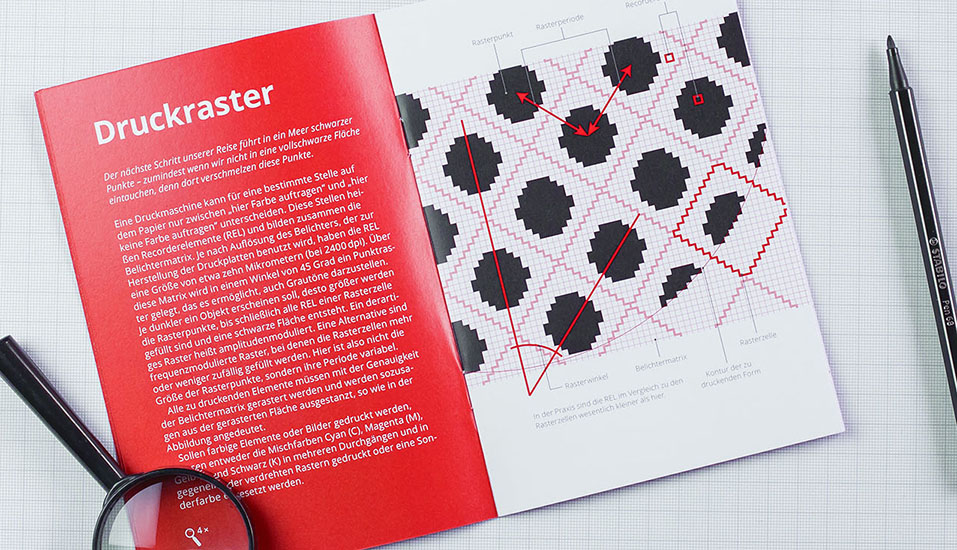
\includegraphics[width=\usedim{eq-col-width}]{img/projects/dekonstruiert}
   }
   \setprojectvar{dekonstruiert}{content}{
      Das Büchlein \emph{Dekonstruiert} nimmt den Leser mit auf eine „Reise ins
      Detail“ und beleuchtet dabei die verschiedensten Aspekte der Buchproduktion vom
      Satzspiegel, über das Druckraster bis hin zu Quanten. Das Büchlein habe ich mit
      Illustrator und InDesign erstellt.
      \projectlink{tobiw.de/illustration}
   }
   
   \setprojectvar{master}{title}{Transmittierte und reflektierte Wellen}
   \setprojectvar{master}{image}{
      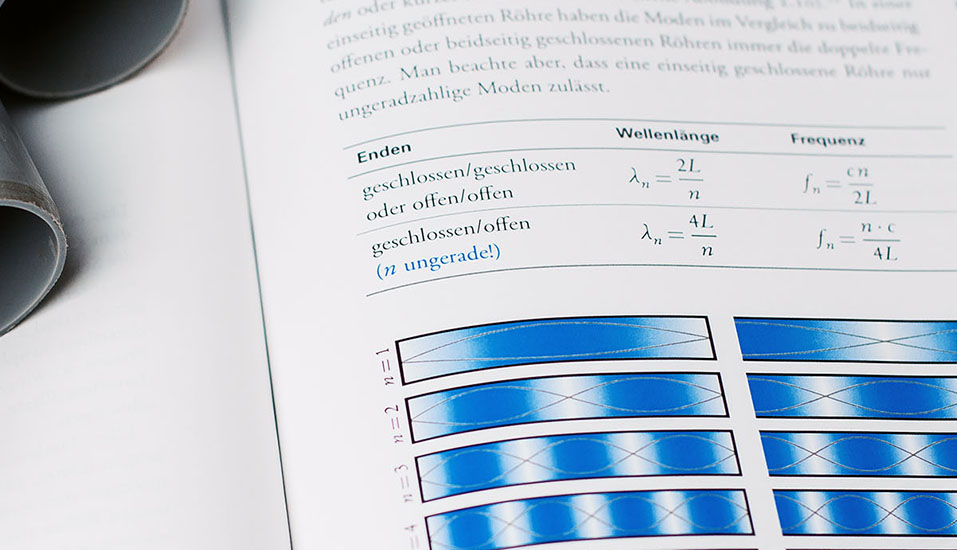
\includegraphics[width=\usedim{eq-col-width}]{img/projects/master_thesis}
   }
   \setprojectvar{master}{content}{
      Zum Abschluss meines Lehramtsstudiums entstand meine Masterarbeit mit dem Titel
      „Anschauliche Erklärung der trans\-mittierten und reflektierten Schallwellen am
      Ende einer offenen Röhre“. Die Arbeit habe ich mit \XeTeX/ gesetzt und mit \TikZ/
      \linebreak illustriert.
      \projectlink{tobiw.de/galerie/schwingungen-und-wellen}
   }
   
   \setprojectvar{metrix}{title}{\LaTeX/-Paket \emph{metrix}}
   \setprojectvar{metrix}{image}{
      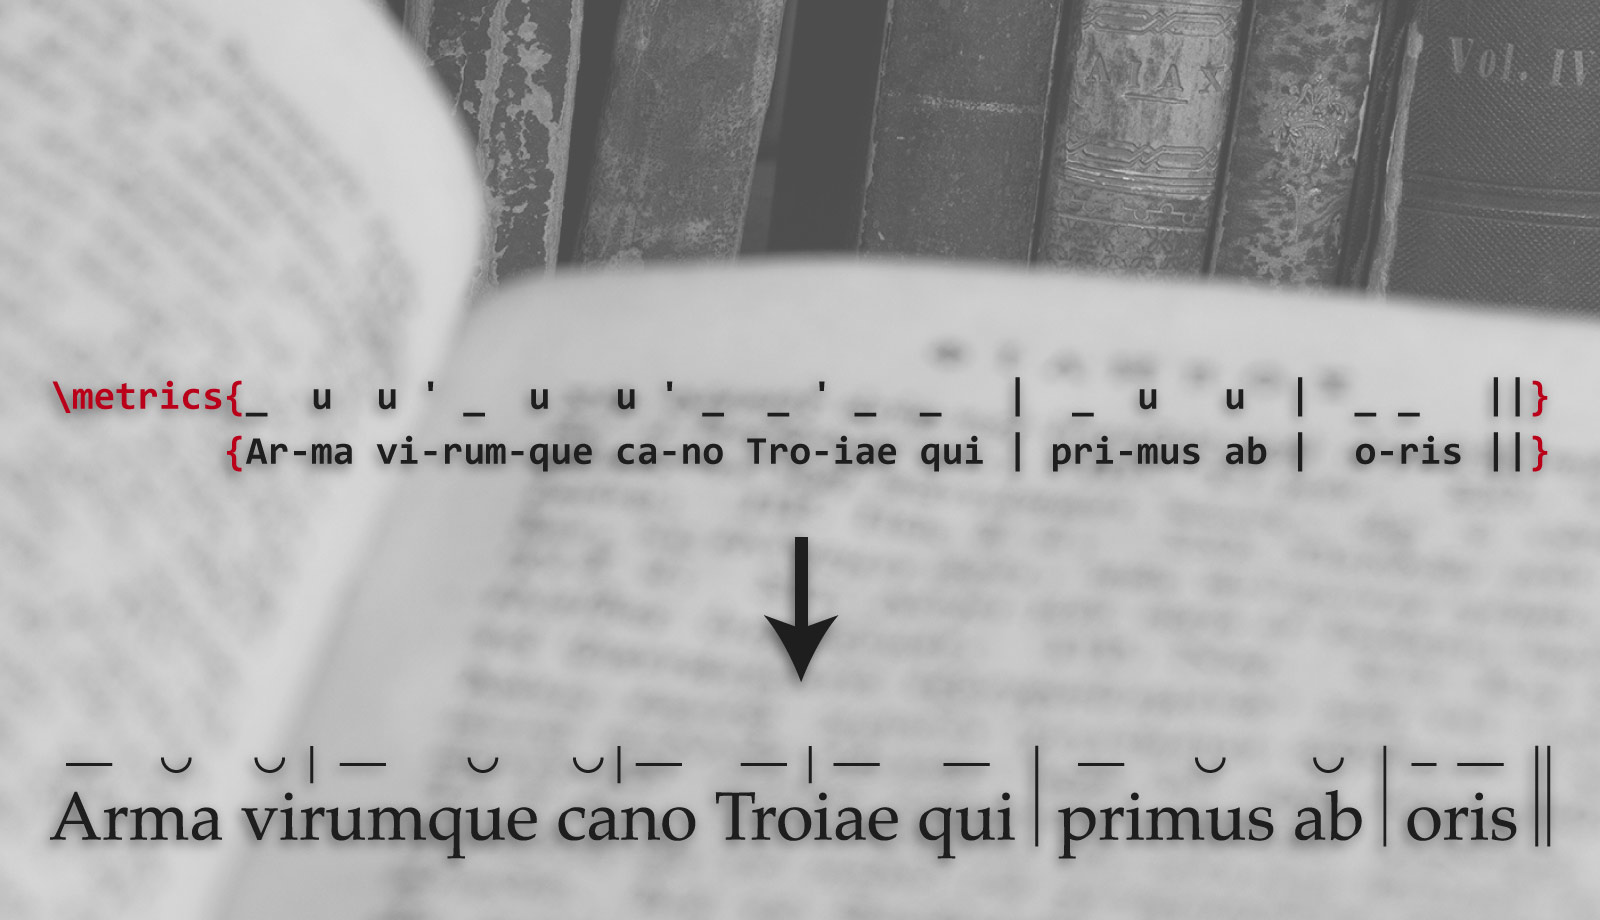
\includegraphics[width=\usedim{eq-col-width}]{img/projects/metrix}
   }
   \setprojectvar{metrix}{content}{
      Das Paket \emph{metrix} dient dazu die Prosodie eines (lateinischen) Verses
      anzugeben, wobei die Ausrichtung der Symbole über den Silben halbautomatisch
      erfolgt. Das Paket habe ich weitestgehend mit den neuen \LaTeXiii/-Funktionen
      implementiert.
      \projectlink{tobiw.de/tex-beratung-und-programmierung\#metrix}
   }
   
   \setprojectvar{mos}{title}{Musikedition Osnabrücker Schloss}
   \setprojectvar{mos}{image}{
      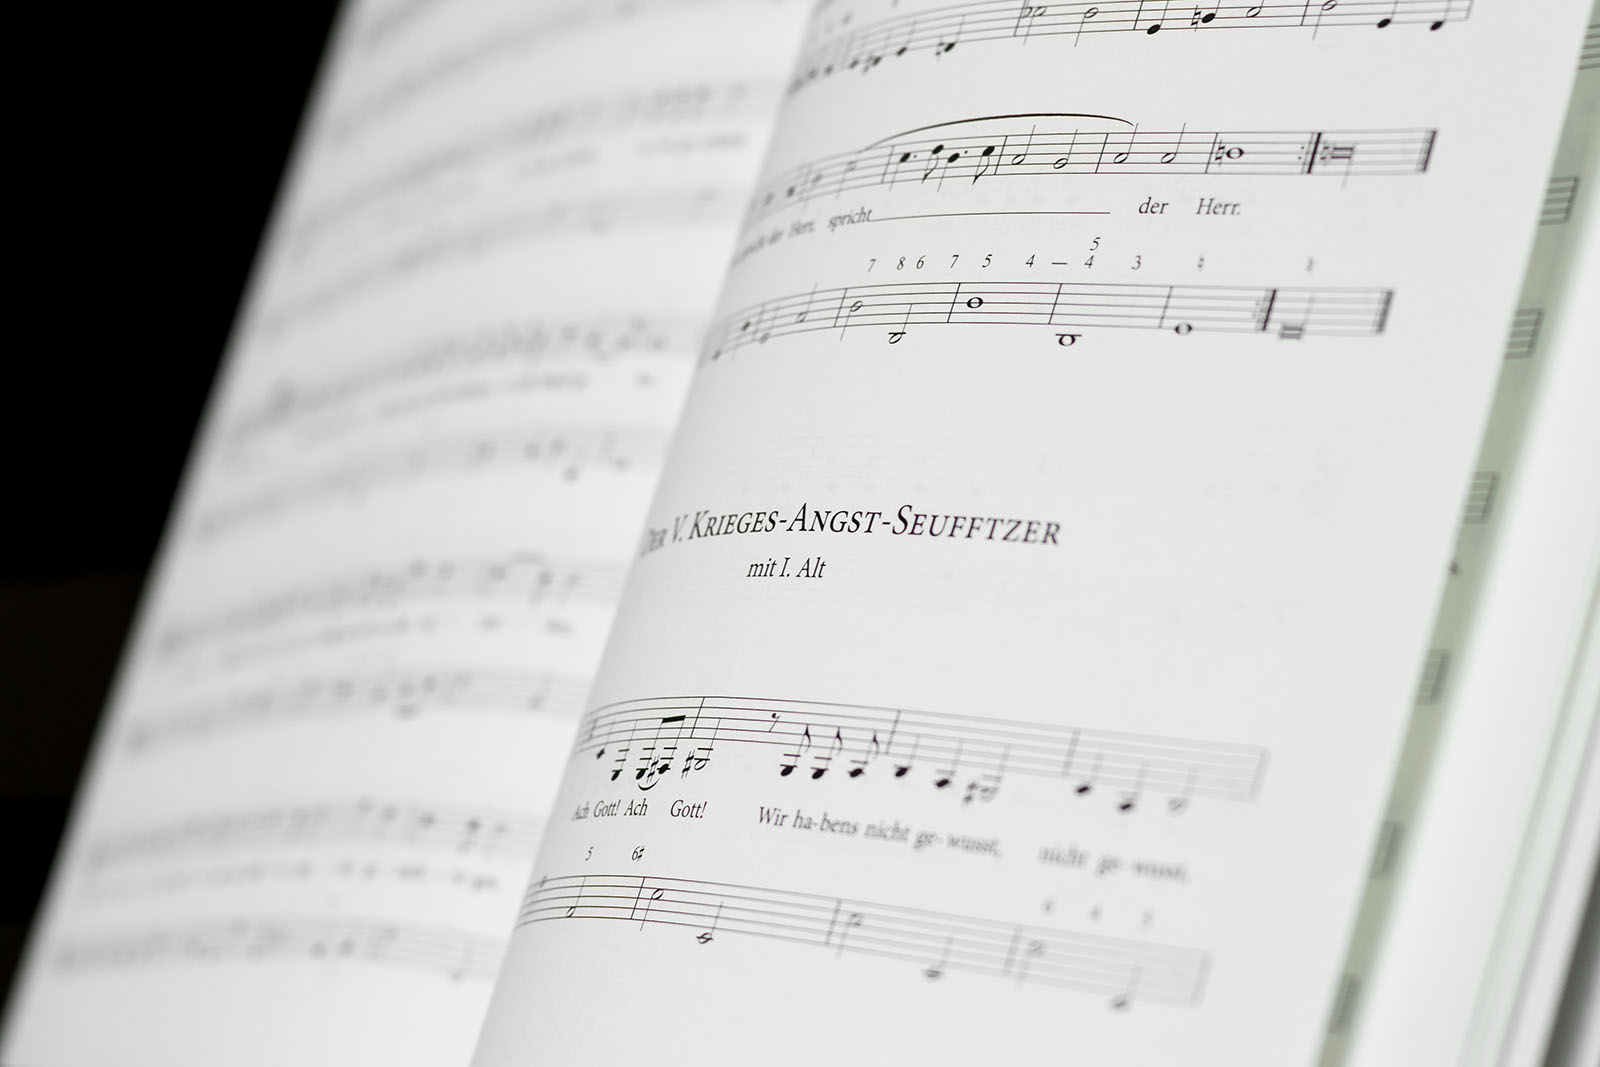
\includegraphics[width=\usedim{eq-col-width}]{img/projects/mos}
   }
   \setprojectvar{mos}{content}{
      Für die 2013 gegründete Reihe für kritische Ausgaben von Noten
      \emph{Musikedition Osnabrücker Schloss} habe ich ein Layout ausgearbeitet und
      den Satz der bisher erschienenen Ausgaben übernommen. Bei der ersten Ausgabe
      war ich außerdem an der\linebreak Edition selbst beteiligt.
      \projectlink{tobiw.de/notensatz}
   }
   
   \setprojectvar{musicaincantans}{title}{Musica Incantans}
   \setprojectvar{musicaincantans}{image}{
      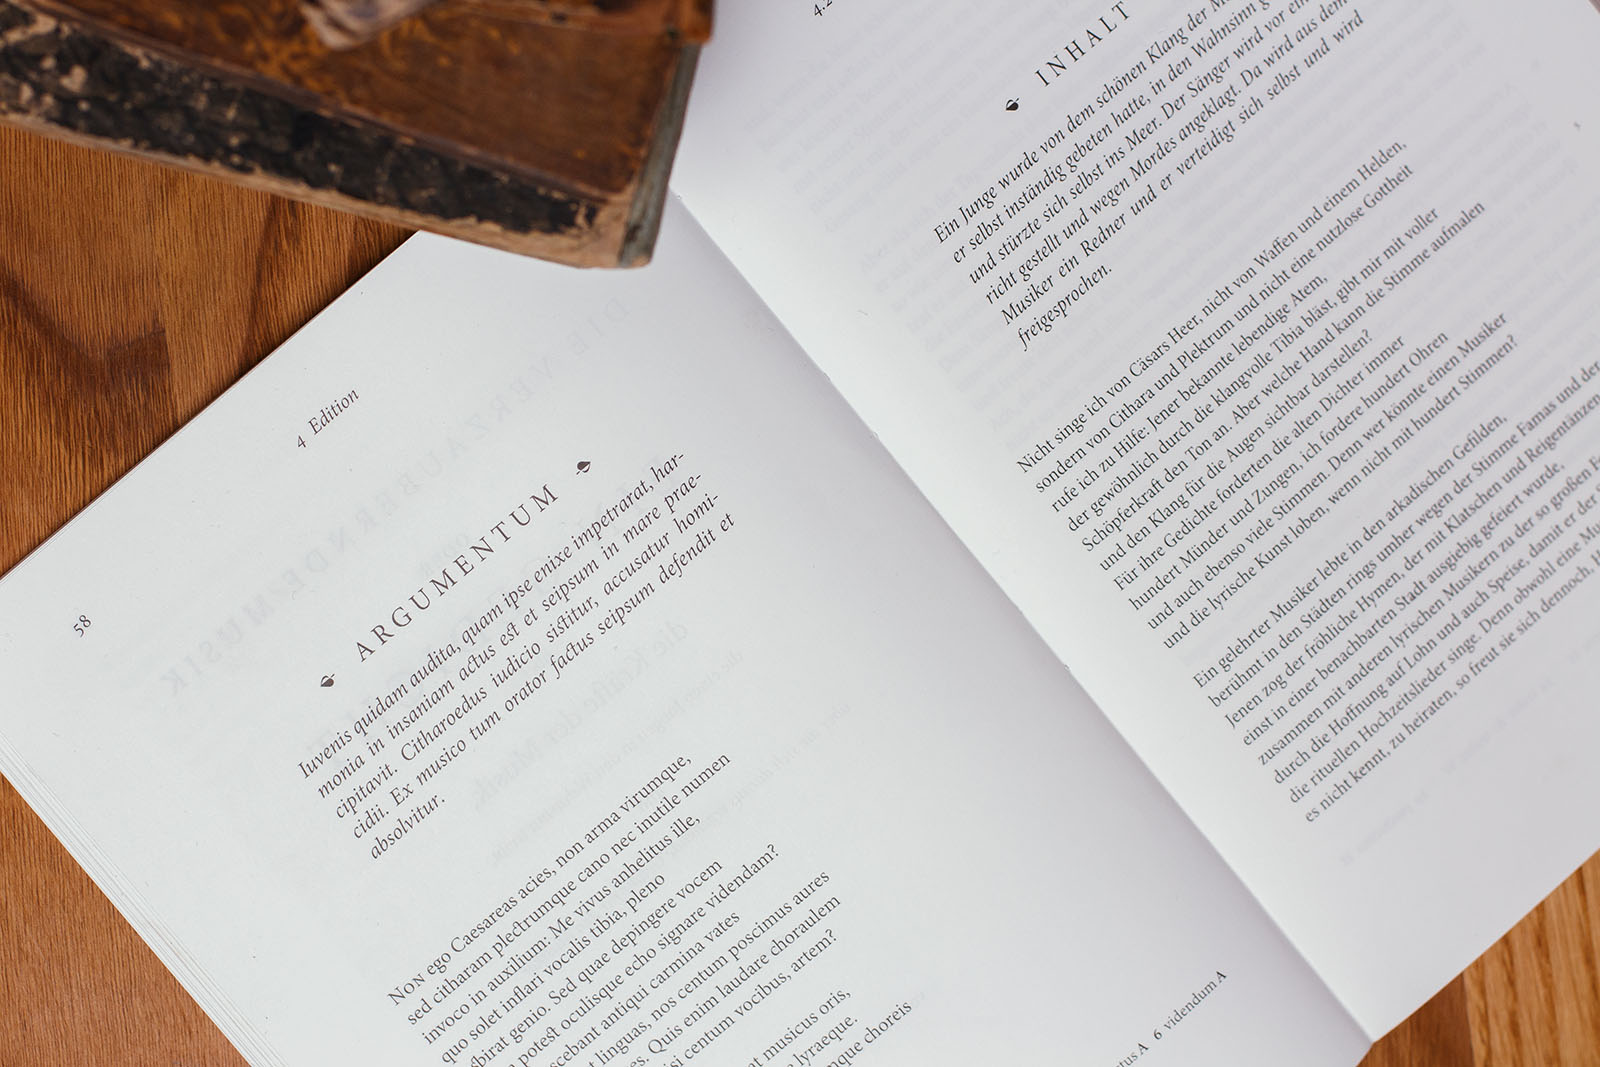
\includegraphics[width=\usedim{eq-col-width}]{img/projects/musica_incantans}
   }
   \setprojectvar{musicaincantans}{content}{
      \emph{Musica Incantans} ist die kritische Ausgabe eines neulateinischen
      Gedichtes von Robert South über die Macht der Musik. Das Gedicht selbst ist auf
      gegenüberliegenden Seiten im Original und in deutscher Übersetzung gedruckt.
      Gesetzt habe ich es mit \XeTeX/.
      \projectlink{tobiw.de/buch-und-textgestaltung}
   }
   
   \setprojectvar{nve}{title}{Niedersächsisches Vokalensemble e.\,V.}
   \setprojectvar{nve}{image}{
      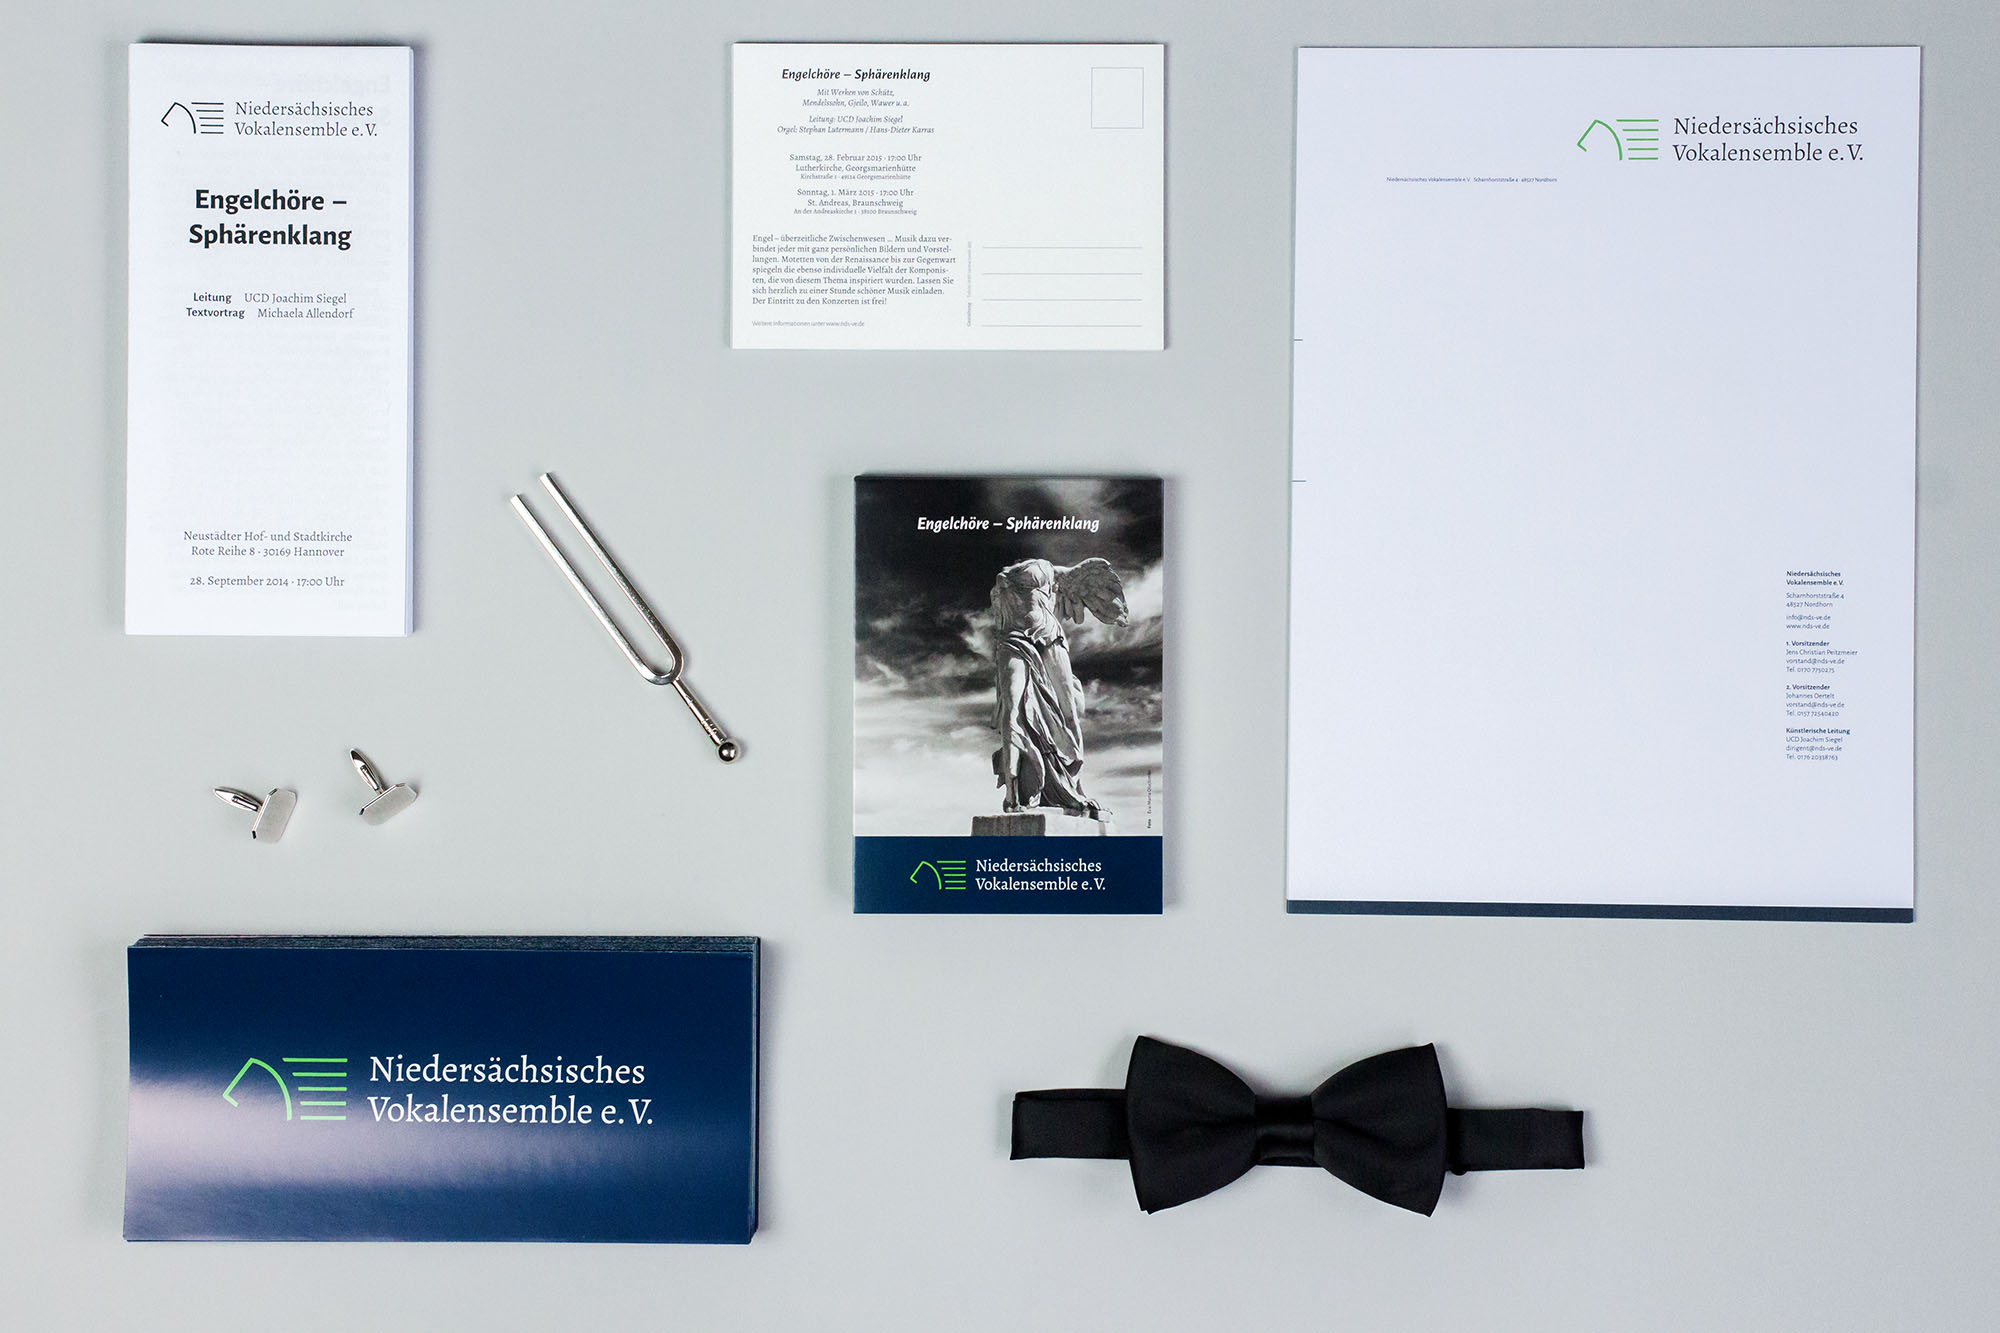
\includegraphics[width=\usedim{eq-col-width}]{img/projects/nve}
   }
   \setprojectvar{nve}{content}{
      Das Niedersächsische Vokalensemble ist ein 2014 ins Leben gerufener,
      Kammerchor, der anspruchsvolle Chormusik von der Renaissance bis zur Moderne
      erarbeitet und aufführt. Ich habe für den Chor ein Corporate Design entwickelt
      und in verschiedenen Medien umgesetzt.
      \projectlink{tobiw.de/corporate-design}
   }
   
   \setprojectvar{speight}{title}{Sam\kern-0.2pt’\kern-0.7pts Mass}
   \setprojectvar{speight}{image}{
      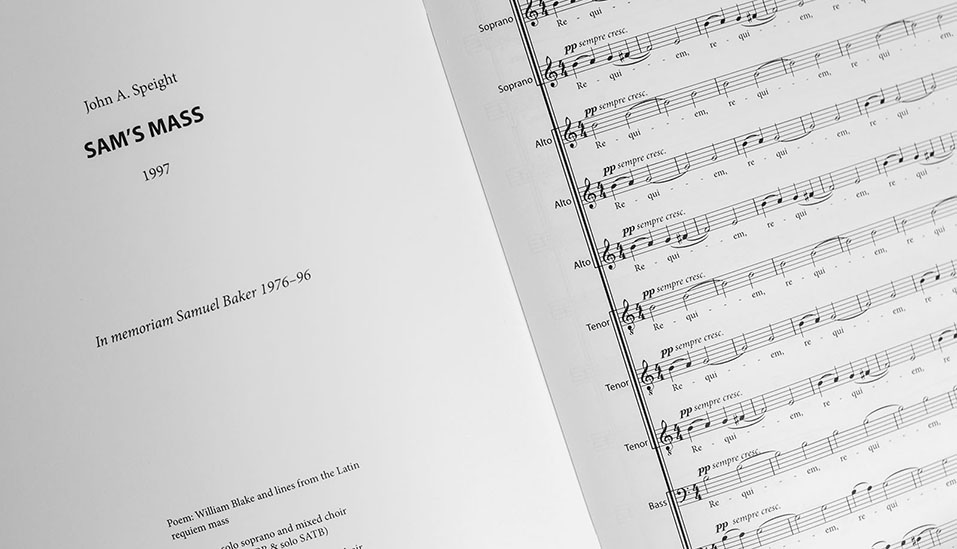
\includegraphics[width=\usedim{eq-col-width}]{img/projects/speight}
   }
   \setprojectvar{speight}{content}{
      Für den Kammerchor der Uni Osnabrück habe ich aus den nur in Handschrift
      erhältlichen Noten von \emph{Sam’\kern-0.6pts Mass} eine leichter lesbare gedruckte
      Version angefertigt, wobei ich zusätzliche Symbole entwickelt habe, um den
      Sängern die Orientierung zu erleichtern.
      \projectlink{tobiw.de/galerie/sams-mass}
   }
\end{languagecontent}

\MakePortfolio[
   dekonstruiert,
   nve,
   musicaincantans,
   metrix,
   master,
   mos%,
%   speight
]

\end{document}